\section{Linear filter design based on selectors}\label{methodology_filtering}

In this section we present the whole methodology which leads to the raw vibration signal enhancement. It is composed of 4 steps (Fig.~\ref{filtering_fig1}):
\begin{itemize}
\item{decomposition of the signal into two-dimensional time-frequency plane,}
\item{selector values calculations for informative band selection,}
\item{estimation of thresholds for individual frequency bins,}
\item{filtering of raw vibration signal and envelope analysis.}
\end{itemize}
At first, the signal is decomposed into a time-frequency map (STFT), which is an estimate of energy fluctuation at particular frequency bins in time. Specifically, we process sub-signals, i.e. time series associated with a particular frequency bin. Each sub-signal is examined how far from Gaussian is its empirical distribution. In order to do this, we examine values of several selectors calculated for every sub-signal. The selectors are based on statistical moments, empirical quantiles and cumulative distribution function. As one of the selectors we use the spectral kurtosis.\\
For a given selector, we obtain a set of weights for the whole signal's spectrum. The weights are used to establish a linear filter similar to the Wiener filter based on the SK~\cite{Combet2009652}. Filtering incorporates the discrete Fourier transform (DFT) and its inverse. In order to enhance filter's amplitude response we propose to cut-off the selector values using individual thresholds for each frequency bin. The thresholds are calculated upon reference signals, whose amplitude spectra are similar to the amplitude spectrum of the raw vibration signal. The reference signals are simulated using the Monte Carlo method and a procedure called inverse pre-whitening.\\
After the thresholds are calculated and selector values are enhanced, we propose to filter the signal in frequency domain. Then, the signal's envelope spectrum is analyzed.
\begin{figure}[!t]
\centering
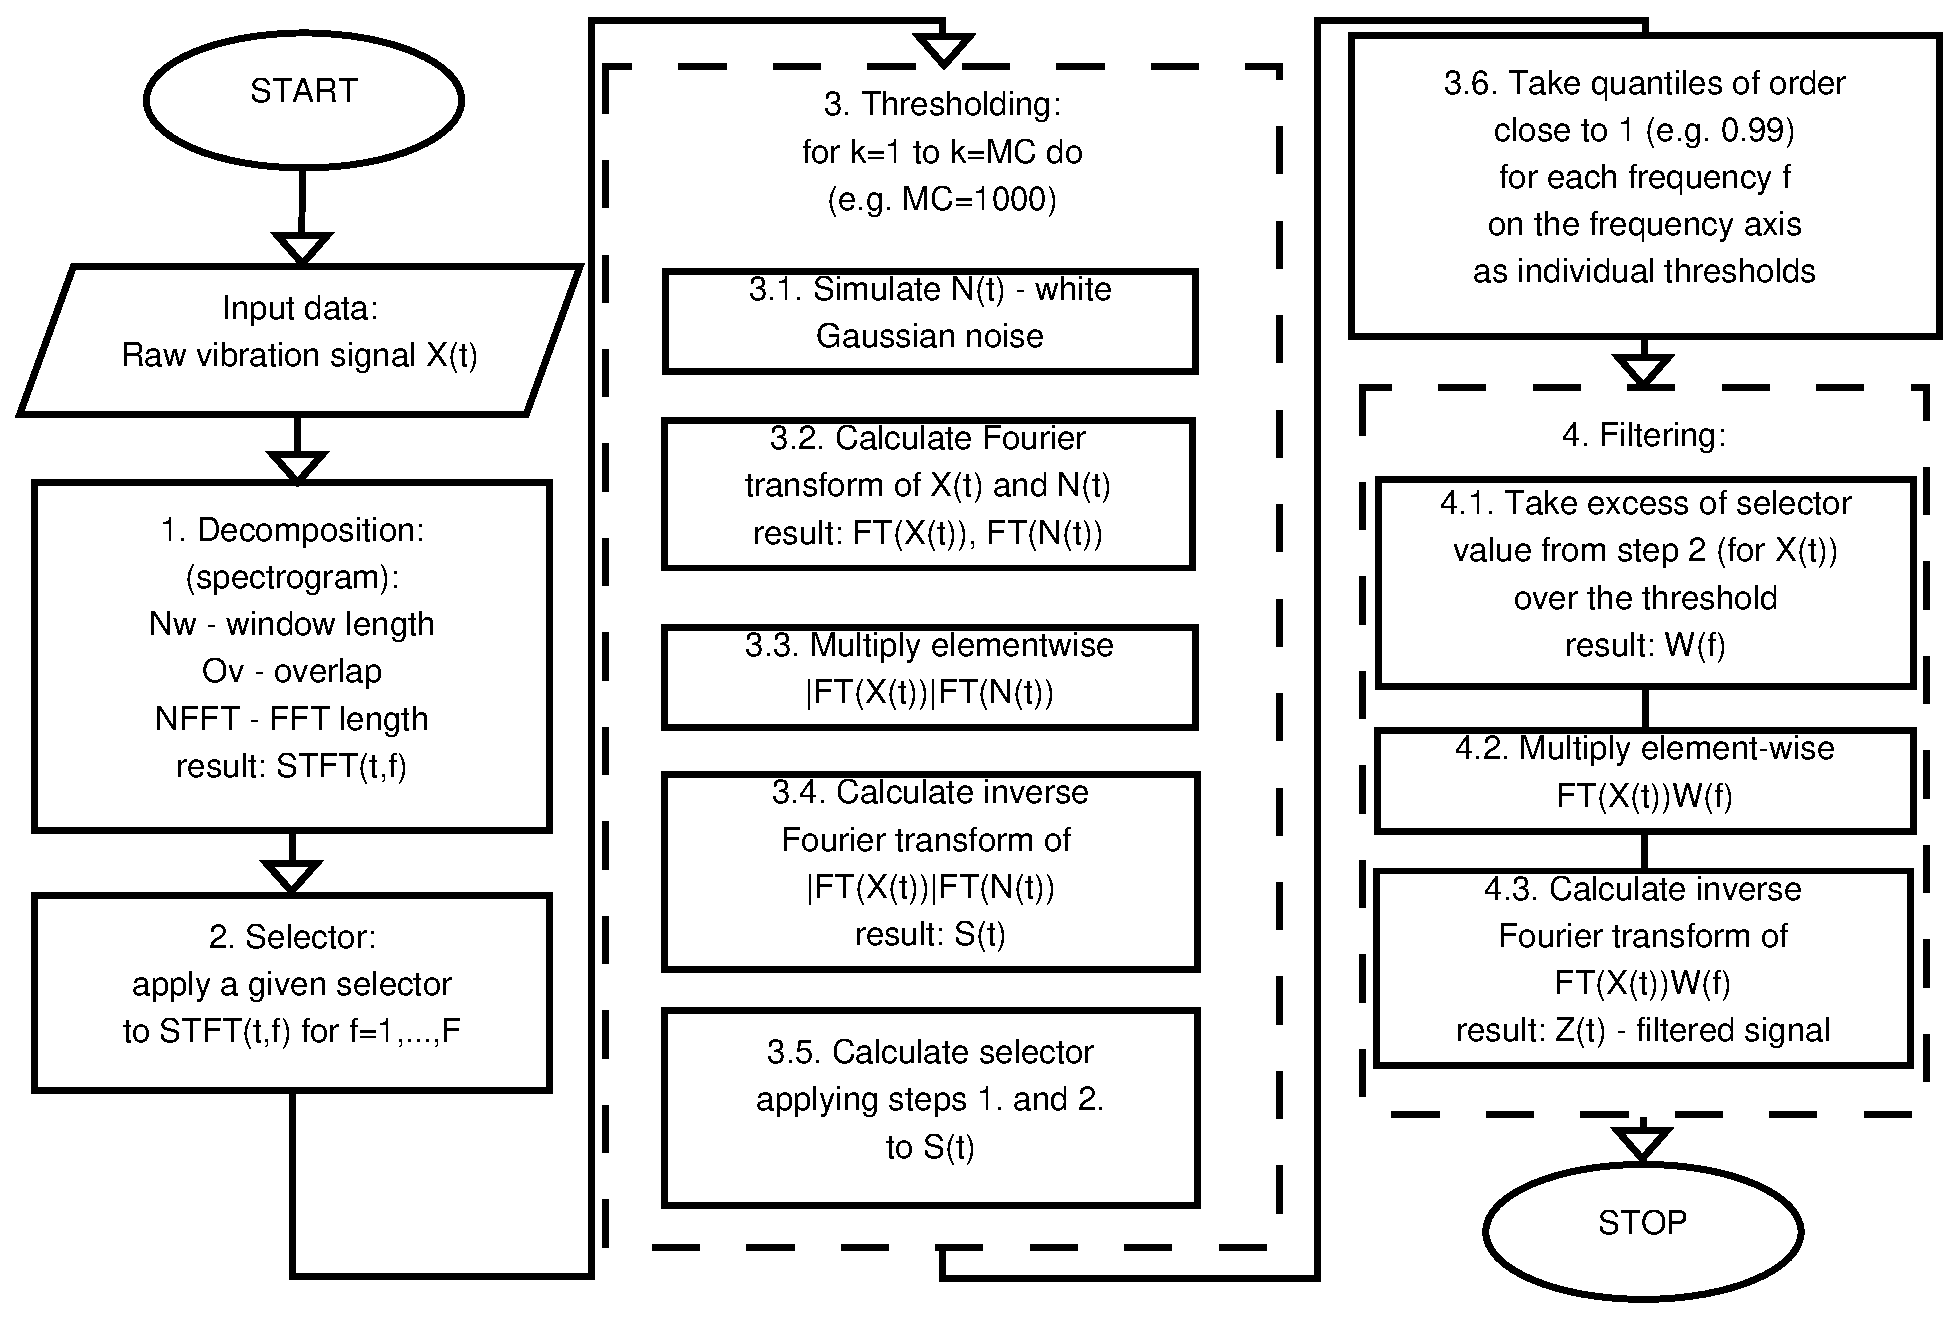
\includegraphics[width=1\textwidth]{methodology/filtering/Diagram2}
\caption{Block diagram of the filtering procedure.}
\label{filtering_fig1}
\end{figure}
\subsection{Decomposition}\label{filtering_decomposition}
Decomposition is based on analysis of the discrete short-time Fourier transform (STFT) which for $x_1,x_2,...,x_N$, time point $t= \left\{1,\ldots,T\right\}$ and frequency $f= \left\{1,\ldots,F\right\}$ is defined as follows~\cite{Allen1977235}:
\begin{eqnarray}
STFT(t,f)=\sum_{k=0}^{N-1}x_k w(t-k)e^{-2j\pi f k/N},
\label{filtering_stft-discr}\end{eqnarray}
where $w(t-k)$ is the shifted window and $x_k$ is the input signal. The window (length and shape) affects the final result in the similar manner as in the spectral kurtosis case. In this paper we present results obtained by using 80\% overlapping.
\subsection{Selectors}\label{filtering_selectors}
In this section we recall four selectors~\cite{Obuchowski2014138,Obuchowski2013441}, each of them could be a base for a linear filter. For comparison, one of the selectors is the classical spectral kurtosis. Recall, that the SK is based on the fourth-order statistic. The spectral kurtosis at the frequency bin $f$ is defined as follows~\cite{Antoni2006308}:
\begin{eqnarray}
SK(f)=T\frac{\sum_{t=1}^{T}|STFT(t,f)|^4}{(\sum_{t=1}^{T}|STFT(t,f)|^2)^2}.\label{filtering_spectral_kurtosis}
\end{eqnarray}
Besides the ability of a pulse train detection, the $SK$ is also very sensitive to a single non-informative impulse that might occur, for instance, during the signal acquisition. In the classical definition, the sum in~(\ref{filtering_spectral_kurtosis}) is reduced by 2 which stands for a cut-off threshold, i.e. only the values of $SK(f)$ larger than 2 are significant. In our approach such subtraction is not necessary - the thresholding procedure quantifies the significance of each selector's value and takes into account only the excess over the threshold.\\
The second selector is the Jarque-Bera statistic~\cite{Jarque1980255,Burnecki2012}. It is based on both kurtosis and skewness. The $JB$ at $f=1,\ldots,F$ is defined as follows:
\begin{eqnarray}
JB(f)=\frac{T}{6}\left(S(f)^2+\frac{\left(K(f)-3\right)^2}{4}\right),
\end{eqnarray}
where $S(f)$ and $K(f)$ are the empirical skewness and kurtosis, respectively, calculated for a given sub-signal, corresponding to the frequency bin $f$. $JB$ exploits not only the fourth, but the third moment as well, in order to examine gaussianity of the random sample. Thus, it might indicate asymmetry of distribution, which occurs in specific types of damage in rotating machines~\cite{Ovacikli2013462}. The higher value of $JB$, the more the distribution of the sample differs from the Gaussian distribution.\\
The next selector is based on a quantile-quantile plot (QQplot). Vertical and horizontal axes of the QQplot are here related to quantiles of empirical sub-signal's distribution and the standard Gaussian distribution, respectively. The selector quantifies the average distance between markers of QQplot and a reference line defined by first and third quartiles of both distributions~\cite{Obuchowski2013441}. The selector $H_{aver}$ at $f=1,\ldots,F$ is defined as~\cite{Obuchowski2014138}:
\begin{eqnarray}
H_{aver}(f)=\frac{1}{T}\sum_{k=1}^{k=T}{ \left| \widetilde{\Phi}^{-1}\left(\frac{2k-1}{2T} \right) - a S(k,f)-b \right| },
\end{eqnarray}
where $\widetilde{\Phi}^{-1}(\cdot)$ is the inverse of cumulative distribution function of the standard Gaussian distribution, i.e. $$\widetilde{\Phi}(x)=\int^{x}_{-\infty} \! \frac{1}{\sqrt{2\pi}}\exp \left( -\frac{x^2}{2} \right) \, \mathrm{d} x,$$ $S(k,f)$ is the $k$-th value of ascending sorted sub-signal $\{|STFT(t,f)|\}_{t=1,\ldots,T}$, $a=\dfrac{\widetilde{\Phi}^{-1}(0.75)-\widetilde{\Phi}^{-1}(0.25)}{q(f,0.75)-q(f,0.25)}$, $b=\widetilde{\Phi}^{-1}(0.75)-aq(f,0.75)$ and $q(f,p)$ is a $p$-th order quantile of a sub-signal $\{|STFT(t,f)|\}_{t=1,\ldots,T}$. In~\cite{Obuchowski2013441} it is shown that this selector distinguishes healthy from faulty bearing's signal as good as SK does, but $H_{aver}$ defines a different order on the set of sub-signals than $SK$ does. Recall that $H_{aver}$ is scale-invariant, since the distance is measured on the axis corresponding to standard normal distribution. Due to the design of $H_{aver}$, one can notice its robustness to single outlying values. One can consider two signals of different lengths, the same statistical distribution and both of them contain a single outlier of similar level. Then $H_{aver}$ is lower for the longer signal, since the appropriate quartiles and $S(k,f)$'s are similar and the denominator, namely $T$, distinguishes these signals.\\
The next selector incorporates the idea of quantifying the distance between the empirical cumulative distribution function (empirical CDF) of the sub-signal and the CDF of the fitted Gaussian distribution. Specifically, it is a Kolmogorov-Smirnov statistic which is defined as follows~\cite{Obuchowski2014138,cordernonparametric,Justel1997251}:
\begin{equation}\label{filtering_K-S}
KSS(f)=sup_x\left|ECDF(f,x)-\Phi(f,x)\right|,
\end{equation}
where $\Phi(f,\cdot)$ is the cumulative distribution function of the Gaussian distribution with mean and variance estimated from the sub-signal corresponding to the frequency bin $f$. Therefore this function is given by:
\begin{eqnarray}\label{filtering_FF}
\Phi(f,x)=\int^{x}_{-\infty} \! \frac{1}{\sqrt{2\pi\widehat{\sigma}(f)^2}}\exp \left( -\frac{\left(x-\widehat{\mu}(f)\right)^2}{2\widehat{\sigma}(f)^2} \right) \, \mathrm{d} x,
\end{eqnarray}
where $\widehat{\mu}(f)$ is the empirical mean of the sub-signal $\{|STFT(t,f)|\}_{t=1,\ldots,T}$, and $\widehat{\sigma}(f)$ is the empirical standard deviation of $\{|STFT(t,f)|\}_{t=1,\ldots,T}$. Moreover, $ECDF(f,x)$ is the empirical cumulative distribution function calculated for the sub-signal corresponding to the frequency bin $f$:
\begin{eqnarray}\label{filtering_ECDF}
ECDF(f,x)=\frac{1}{T}\sum_{t=1}^{T}\mathbf{1}\left\{ |STFT(t,f)|\leq x\right\}.
\end{eqnarray}
In the above definition $\mathbf{1}\{a\leq x\}$ denotes the indicator function, i.e. $\mathbf{1}\{a\leq x\}=1$ if $a\leq x$ and 0 otherwise. This selector is also scale-invariant. Moreover, in opposite to the previous selectors, $KSS$ is bounded since values of both cumulative distribution functions (i.e. $ECDF$ and $\Phi$) are between 0 and 1.\\
The values of a particular selector for the entire spectrum constitute a ground for the amplitude response of the filter. The following sections provide a complete description how to obtain the final filter that might be used to obtain the informative part of the vibration signal.
\subsection{Thresholding}\label{filtering_thresholding}
Once the amplitude response of the filter is calculated, it has to be enhanced in order to take into account the significant values of the selector only. We propose to design significance thresholds for each frequency bin individually.
\begin{figure}[!ht]
\begin{center}
\includegraphics[width=0.49\textwidth]{methodology/filtering/sin_const-quantile_lines_g}
\includegraphics[width=0.49\textwidth]{methodology/filtering/sin_const-quantile_lines_b}
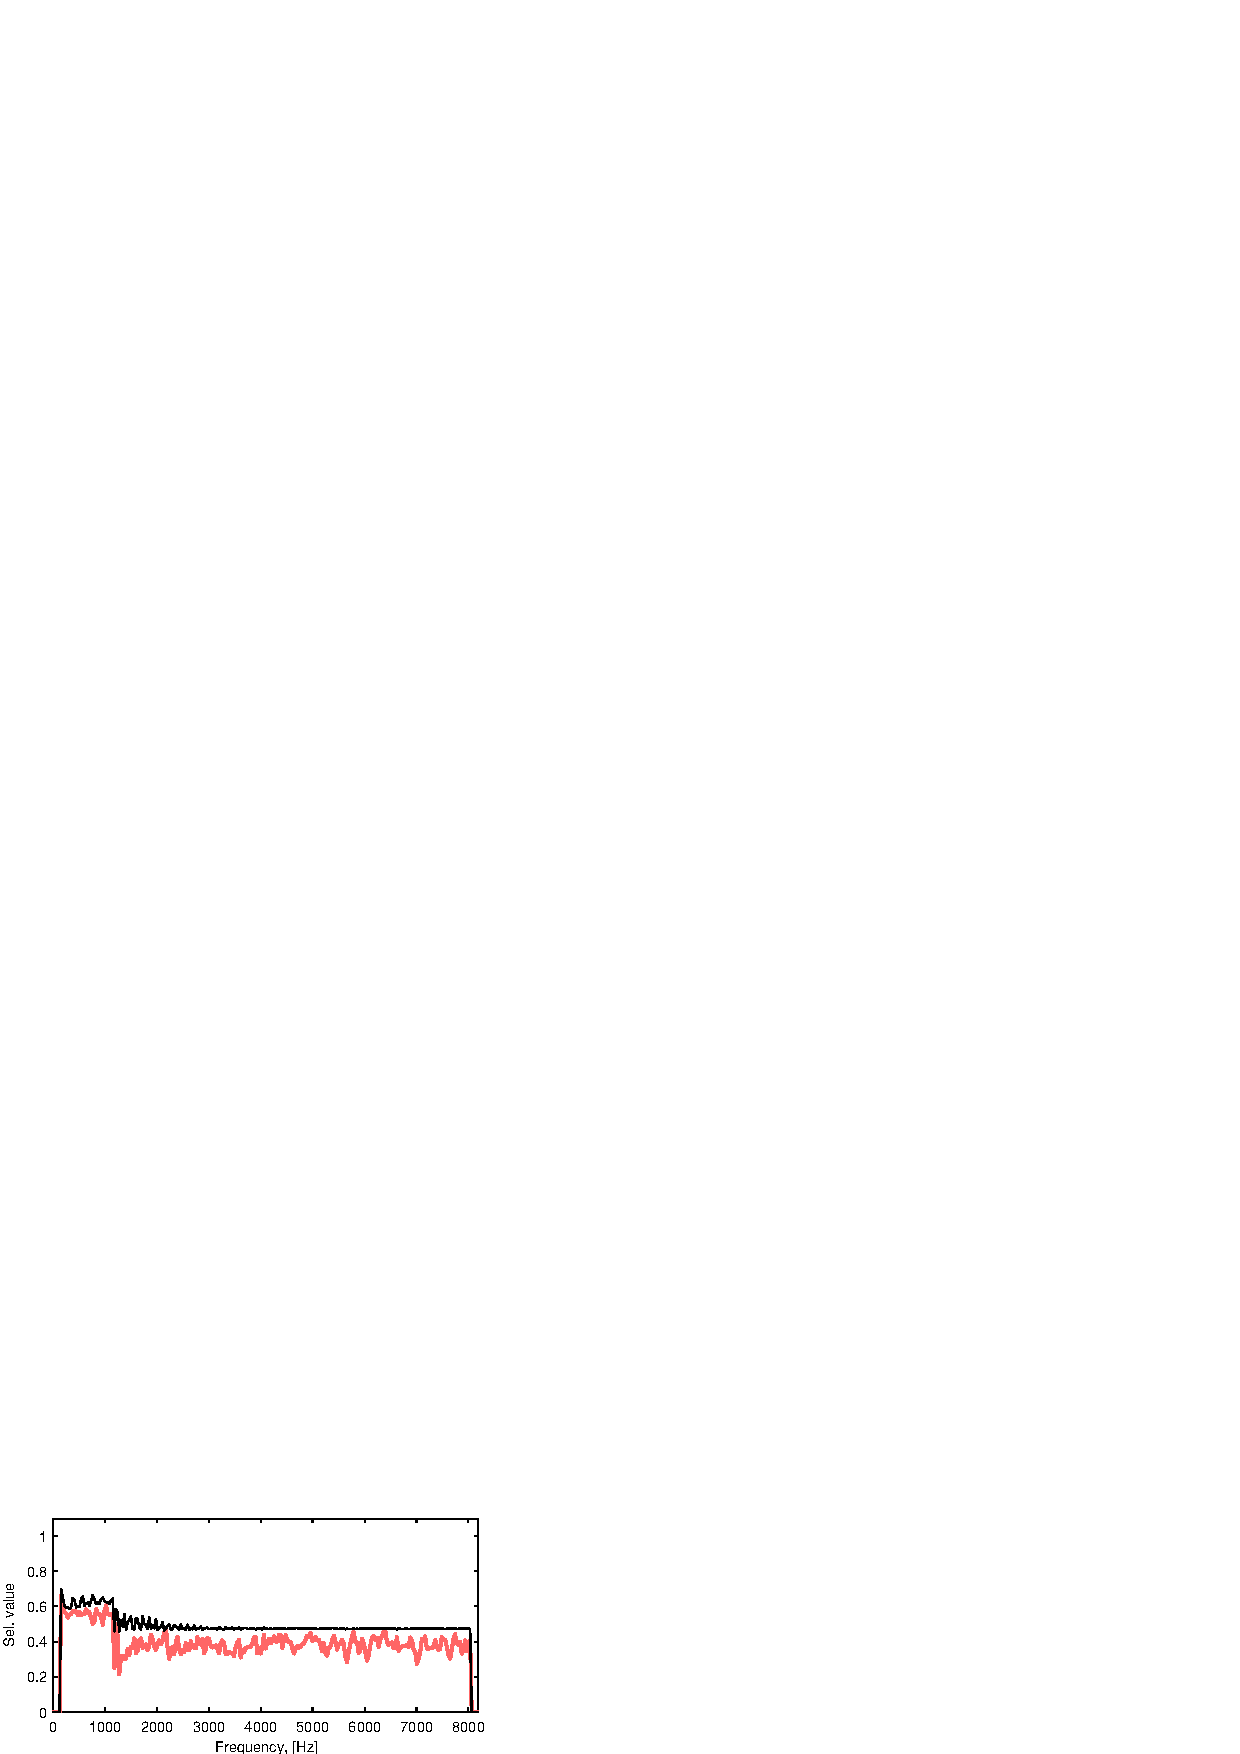
\includegraphics[width=0.49\textwidth]{methodology/filtering/sin_const-quantile_99_g}
\includegraphics[width=0.49\textwidth]{methodology/filtering/sin_const-quantile_99_b}
\caption{Selector values of reference signals. Faulty (right panels) and healthy machine (left panels). Red thick lines represent selector values based on $H_{aver}$. Top panels present quantile lines of orders: 0.1, 0.3, 0.5, 0.7 and 0.9 (black thin lines) obtained upon selector values of 1000 reference signals. Bottom panels present significance thresholds for the selector values, i.e. quantile of order 0.99. Note that only at a few frequency bins selector values for healthy machine exceeds the threshold and the threshold is significantly exceeded at 2000-7000~Hz for faulty machine.\label{filtering_sim-selekt}}
\end{center}
\end{figure}
This step is essential when energy contained in the informative frequency band is relatively low, i.e. the signal also contains high-energy components that do not carry information about the local damage. In order to illustrate this point, consider a vibration signal that consists of: a) high-energy low-frequency component (component related to normal operation of the machine), b) low-energy component located at the half of the frequency range (component related to local damage) and c) low-energy noise located at the highest frequency bands (non-informative from diagnostic point of view). Values of any selector (that indicates impulsivity) at low frequency bands (not related to damage) are significantly lower than selector values at middle frequency bands (related to local damage). Thus, the signal filtered using such selector might still be affected by the low-frequency component. In other words, high spectral amplitudes of low-frequency signal components multiplied by low selector values might be still larger than low amplitudes (located at informative, middle frequency bands) multiplied by a high values of the selector. Thus, the whole procedure might provide unsatisfactory results, i.e. energy of non-informative components will dominate in the filtered signal.\\
Another reason describing benefits of thresholding is derived from analysis of a signal that consists of the high-energy low-frequency component and the noise only. It might happen that selector values at low frequency bands, containing high-energy  deterministic content, are different from values at frequency bands containing noise (with relatively low energy). Such case might be caused by specific windowing, e.g. when the STFT window length is not large enough to appropriately estimate energy flow at low frequency bands. Fig.~\ref{filtering_sim-selekt} illustrates this point. The signals $r_1(t)$ and $r_2(t)$ presented therein are sums of 6 sine waves with frequencies $190n$~Hz, $n=1,\ldots,6$ and a noise dependent on whether the signal from faulty or healthy machine is simulated. The signals $\left\{r_k(t)\right\},\,k=1,2$ are obtained using the following formula:
\begin{eqnarray}
r_k(t)=\sum^{N}_{n=1}{ A a_n \sin(2\pi f_n t)} + \sigma m_k(t),
\end{eqnarray}
where $N=6$, $A=10$, $a_n=0.75^{(n-1)}$, $f_n=190n$, $\sigma=0.1$ and $\left\{m_k(t)\right\},\,k=1,2$ is the noise. The signal from a healthy machine corresponds to the noise $m_1(t)$, which basically is a zero-mean white Gaussian noise with standard deviation equal to 1. $m_2(t)$ is related to a faulty machine and structure of this signal is more complicated. In order to construct $m_2(t)$ we decompose the signal $m_1(t)$ by filtering into 3 components: a) $\left\{m_{1a}(t)\right\}$ - low-pass filtered $\left\{m_1(t)\right\}$ with cut-off frequency 2000~Hz, b) $\left\{m_{1b}(t)\right\}$ - bandpass filtered $\left\{m_1(t)\right\}$ with cut-off frequencies 2000~Hz and 7000~Hz and c) $\left\{m_{1c}(t)\right\}$ - high-pass filtered $\left\{m_1(t)\right\}$ with cut-off frequency 7000~Hz. We use ideal filters, i.e. filters with characteristics equal to 1 along the passed band and 0 elsewhere. Then, we modulate amplitude of $\left\{m_{1b}(t)\right\}$ using an impulsive signal - sum of 128 sine waves with frequencies that are multiples of the fault frequency - $13$~Hz. As a result, the amplitude of the signal between impulses becomes similar to the corresponding amplitude of $\left\{m_1(t)\right\}$. Signal to noise ratio defined as $\mathrm{SNR_{dB}} = 10 \log_{10} \left ( \frac{P_\mathrm{signal}}{P_\mathrm{noise}} \right )$, where $P_\mathrm{signal}$ denotes power of $\sigma m_k(t)$ and $P_\mathrm{noise}$ - power of $\sum^{N}_{n=1}{ A a_n \sin(2\pi f_n t)}$, equals to -42.53~dB in healthy case ($m_1(t)$) and -36.21~dB in faulty case ($m_2(t)$). Frequency sampling is $16384$~Hz and length of the signals is $2.5$~s. The time-frequency map that provides sub-signals is calculated using 133-sample-long Kaiser windows ($\beta=5$) and discrete Fourier transform calculated in 512 points. It can be noticed that values of $H_{aver}$ at low frequency bands are different than values of $H_{aver}$ at middle and high frequency bands. Thus, we claim that each single frequency bin should be thresholded individually.\\
The proposed thresholding procedure is inspired by so called "pre-whitening". Pre-whitening is a method that flattens frequency spectrum of the examined signal~\cite{Sawalhi2005231,Sawalhi2011549,Sawalhi2011846}. Formula for the pre-whitened version of a signal $x(t)$ is~\cite{Borghesani2013370}:
\begin{equation}
y(t)=IDFT\left\{\frac{DFT\left(x(t)\right)}{\left|DFT\left(x(t)\right)\right|}\right\},
\end{equation}
where $DFT$ and $IDFT$  indicate the discrete Fourier transform and its inverse. Frequency spectrum of a signal processed using pre-whitening is flat, but the signal might still contain spikes related to local damage. When the damage signature is weak, the pre-whitened signal might be dominated by noise from frequency bands outside the informative frequency band. Thus, there is a need for enhancement of the pre-whitened signal.\\
We use an inverse of pre-whitening in order to simulate a large number of signals without transients (so called reference signals), but keeping the amplitude spectrum similar to the real data's frequency spectrum. Basically, we multiply absolute value of discrete Fourier transform of the examined signal (e.g. $r_k(t)$ or real data) element-wise by discrete Fourier transform of white noise, i.e. $DFT\left\{n(t)\right\}$, where $n(t)$ is a vector of independent identically distributed Gaussian random variables with mean $\mu=0$ and variance $\sigma^2=1$. Length of $n(t)$ is the same as length of the examined signal. Then, we return to time domain using inverse discrete Fourier transform. The formula for a simulated signal without transients is:
\begin{equation}
s(t)=IDFT\left\{{\left|DFT\left(p(t)\right)\right|}{DFT\left(n(t)\right)}\right\},
\end{equation}
where $p(t)$ is the examined signal and the multiplication is performed element by element. Next, we calculate values of the selector for each reference signal $s(t)$.\\
The procedure is repeated with a lot (e.g. 1000) of different $n(t)$'s (so called Monte Carlo method), thus we obtain a significant number of selector values for each frequency bin. Finally, a certain quantile (e.g. $99\%$) is calculated individually for every $f$. If the selector value at $f$ is lower than the quantile, it is said to be insignificant and set to 0. Otherwise, only the excess over the quantile is taken for final design of the filter.\\
Fig.~\ref{filtering_coloring-stft} in Sec.~\ref{results_filtering_real_data} presents a spectrogram of a vibration signal from a locally damaged heavy rotating machine (a two-stage gearbox from a mining company) and a spectrogram of an exemplary realization of the simulated signal $s(t)$. One can see that both signals share similar content along frequency axis, but the simulated one has no wide-band excitations related to local damage.
\subsection{Filtering}
In the final step we propose to follow the approach presented in~\cite{Combet2009652}, where the optimal Wiener filter based on the $SK$ is described. Recall, that the filter is proportional to the square root of the $SK$. We propose to follow this approach to the selectors proposed in Sec.~\ref{filtering_selectors} and replace square root of the $SK$ by square root of selector values that remains after filter's amplitude response enhancement (thresholding). We also normalize these square roots by their maxima in order to make visual comparison of them easier.\\
Firstly, the discrete Fourier transform of the examined signal is calculated and the filter's amplitude response obtained in Sec.~\ref{filtering_thresholding} is interpolated at all the frequency bins of the discrete Fourier transform. Next, the discrete Fourier transform is multiplied element-wise by the interpolated frequency characteristic. Finally, the inverse discrete Fourier transform is used in order to return to the time domain. The formula for the filtered signal $z(t)$ is as follows:
\begin{equation}
z(t)=IFT\left\{{FT\left(x(t)\right)}{W(f)}\right\},
\end{equation}
where $W(f)$ is the amplitude response of the filter driven by a given selector (e.g. $SK(f)$, $KSS(f)$, $H_{aver}(f)$, etc.), i.e. square root of thresholded values of the selector, interpolated to make the size of $W(f)$ equal to the size of discrete Fourier transform of $x(t)$.
\FloatBarrier
\subsection{Discussion}\label{methodology_filtering_discussion}

In this section we discuss motivation and properties of the proposed methodology and compare it with existing methods. The novelty of the paper is contained mainly in the extension of SK-based filtering (including the thresholding procedure), thus we discuss other methods of one dimensional clustering that might be found in the literature. One dimensional methods of clustering are significantly different from multidimensional ones. The 1D real-valued data is only a special case of multidimensional data, but the difference is in natural ordering of real numbers. All of the discussed methods benefit from this property. The fundamental problem is to distinguish between significant and insignificant values of a particular selector. Thus, there is a need for clustering values of the selector into two groups only.\\
The classical approach for filtering based on the spectral kurtosis (calculated from the STFT) is to subtract 2 from calculated fourth-order statistic and then take only excess over a given significance level $\alpha$, which is proportional to the given quantile of the normal distribution~\cite{Combet2009652,Antoni2006308}. While applying other impulsivity criteria (selectors) to the signal, one can derive analogous thresholds for each single selector. On the other hand, one can simply exploit one of the existing 1D thresholding procedures. We recall and analyze only a few of them, because comparing thresholding methods is not the goal of this paper.\\
In 1979 N. Otsu proposed a method for finding the threshold that minimizes the variance within the group, namely a weighted sum of each group's variances, where weights are just the number of elements in a particular group divided by the number of all thresholded values~\cite{Otsu197962}. In order to calculate this variance-minimizing threshold it is proposed to calculate firstly the variance within the group, taking as the threshold each element of the entire set in the sequence. Then, the final threshold is the argument which minimizes the variance within the group. In our case, where the entire set of selector values is denoted by $\left\{W(f),\,f\in \left\{ 1,\ldots,F\right\}\right\}$ it is only needed to calculate, for each $f_i\in \left\{ 1,\ldots,F\right\}$, the weighted average of variances of each of two groups - one constituted from elements of $\left\{W(f)\leq W\left(f_i\right),\,f\in \left\{ 1,\ldots,F\right\}\right\}$  and $\left\{W(f) > W\left(f_i\right),\,f\in \left\{ 1,\ldots,F\right\}\right\}$. Then, $f_i$ that maximized the weighted sum of variances is the final threshold. Such method is known for setting the threshold close to the component with larger class probability or larger class variance~\cite{Hou20061732}, thus it might fail if only a small frequency band is non-informative (with low values of $W(f)$) and values of $W(f)$ at other frequency bands are much higher and scattered. Then, the threshold might be too high, what results in ignoring some of the informative frequency bins. Recently, a new method for such heavy-tailed 1D data classification called "head/tail breaks" has been proposed by B. Jiang~\cite{Jiang2013482}. In order to avoid the effect of threshold shifting through the right tail of the data, it is proposed to iteratively constitute breakpoints (thresholds). Each breakpoint divides a set into two subsets - one above and one below the breakpoint. These breakpoints are just arithmetic means of the considered set, thus in the first step the arithmetic mean $\mu_1$ of all values in $\left\{W(f),\,f\in \left\{ 1,\ldots,F\right\}\right\}$ is calculated. Then, the mean $\mu_2$ of values above $\mu_1$ is calculated, and so on. In our case, where $\left\{W(f),\,f\in \left\{ 1,\ldots,F\right\}\right\}$ has to be divided into two groups only, this method might provide unsatisfactory results when, for instance, there are just a few values of the selector at IFB much higher than others therein, and low values at non-informative frequency band are present, as usual. Arithmetic mean is known to be sensitive to outliers, thus, once again, some of informative components might be omitted. To sum up, both methods are interesting since they do not assume specific distribution of the data. However, they might omit some informative components, for which corresponding values of the selector are not the largest, but still are significant. This remark led us to invent the thresholding method described in Sec.~\ref{filtering_thresholding}. This one might be applied not only to the kurtosis calculated from the spectrogram, but also to other selectors, for which taking a given quantile of Gaussian distribution is not a method proved as efficient. The only thing we assume is that the reference signal which imitates the same signal as the investigated one, but without local damage, might be simulated using the inverse pre-whitening. Using a number of such simulated signals it can be examined, whether our investigated machine significantly differs from a healthy one or not. Additional advantage of this method is its insensitivity to windowing, i.e. when a particular STFT windowing method provides unlikely high values of a selector for some frequency bands, the method adapts and makes the threshold higher at these bands. One can also make the procedure closer to the reality, i.e. when an appropriate (large) number of signals representing the same measurement related to a healthy machine, might be acquired. Since this extension might be performed well in a laboratory, its application to an industrial case might be difficult.
\FloatBarrier